\documentclass[mathserif]{beamer}
\usepackage{amsmath,amssymb,times,listings,hyperref,url,graphicx,subcaption,placeins,siunitx,enumerate,pdfpages}
\usepackage{subcaption}

\title{Bicycle Wheel System Identification and Optimal Truing Algorithm}
\author{Aaron Hunter}
\date{October 7, 2019}

\usetheme{PaloAlto}
\beamertemplatenavigationsymbolsempty

\begin{document}

\maketitle

\begin{frame}
    \frametitle{Table of Contents}
    \tableofcontents
\end{frame}

\section{Introduction}
  \begin{frame}{Introduction}
    \begin{itemize}
        \item Wheel `truing' is the process of adjusting spoke tension to minimize lateral and radial variations
        \item Commercial robotic bicycle wheel truing machines use a heuristic truing method.  
        \item This method mimics the actions a human might take to perform the task.
        \item This method can be inefficient or ineffective requiring human intervention
    \end{itemize}
     The work that follows demonstrates an optimal approach to wheel truing using system identification techniques and feedback control to achieve wheel alignment. 
  \end{frame}
    
\section{Background}

\begin{frame}{The Bicycle Wheel}
    \begin{itemize}
    \item The bicycle wheel is a structure consisting of a rim, a hub, and spokes connecting the hub to the rim
    \item The spokes are under tension to provide the stiffness to wheel structure
    \item The rim is under compression
    \item The wheel can be considered a system of springs in parallel and series combinations
    \item Spoke tension must be high enough to support the load (bicycle and rider) but not so high that the rim warps laterally
    \item Spokes patterns vary from radial to nearly tangential
    \end{itemize}
\end{frame}

\begin{frame}{Bicycle Wheel Geometry}
    \begin{center}
    	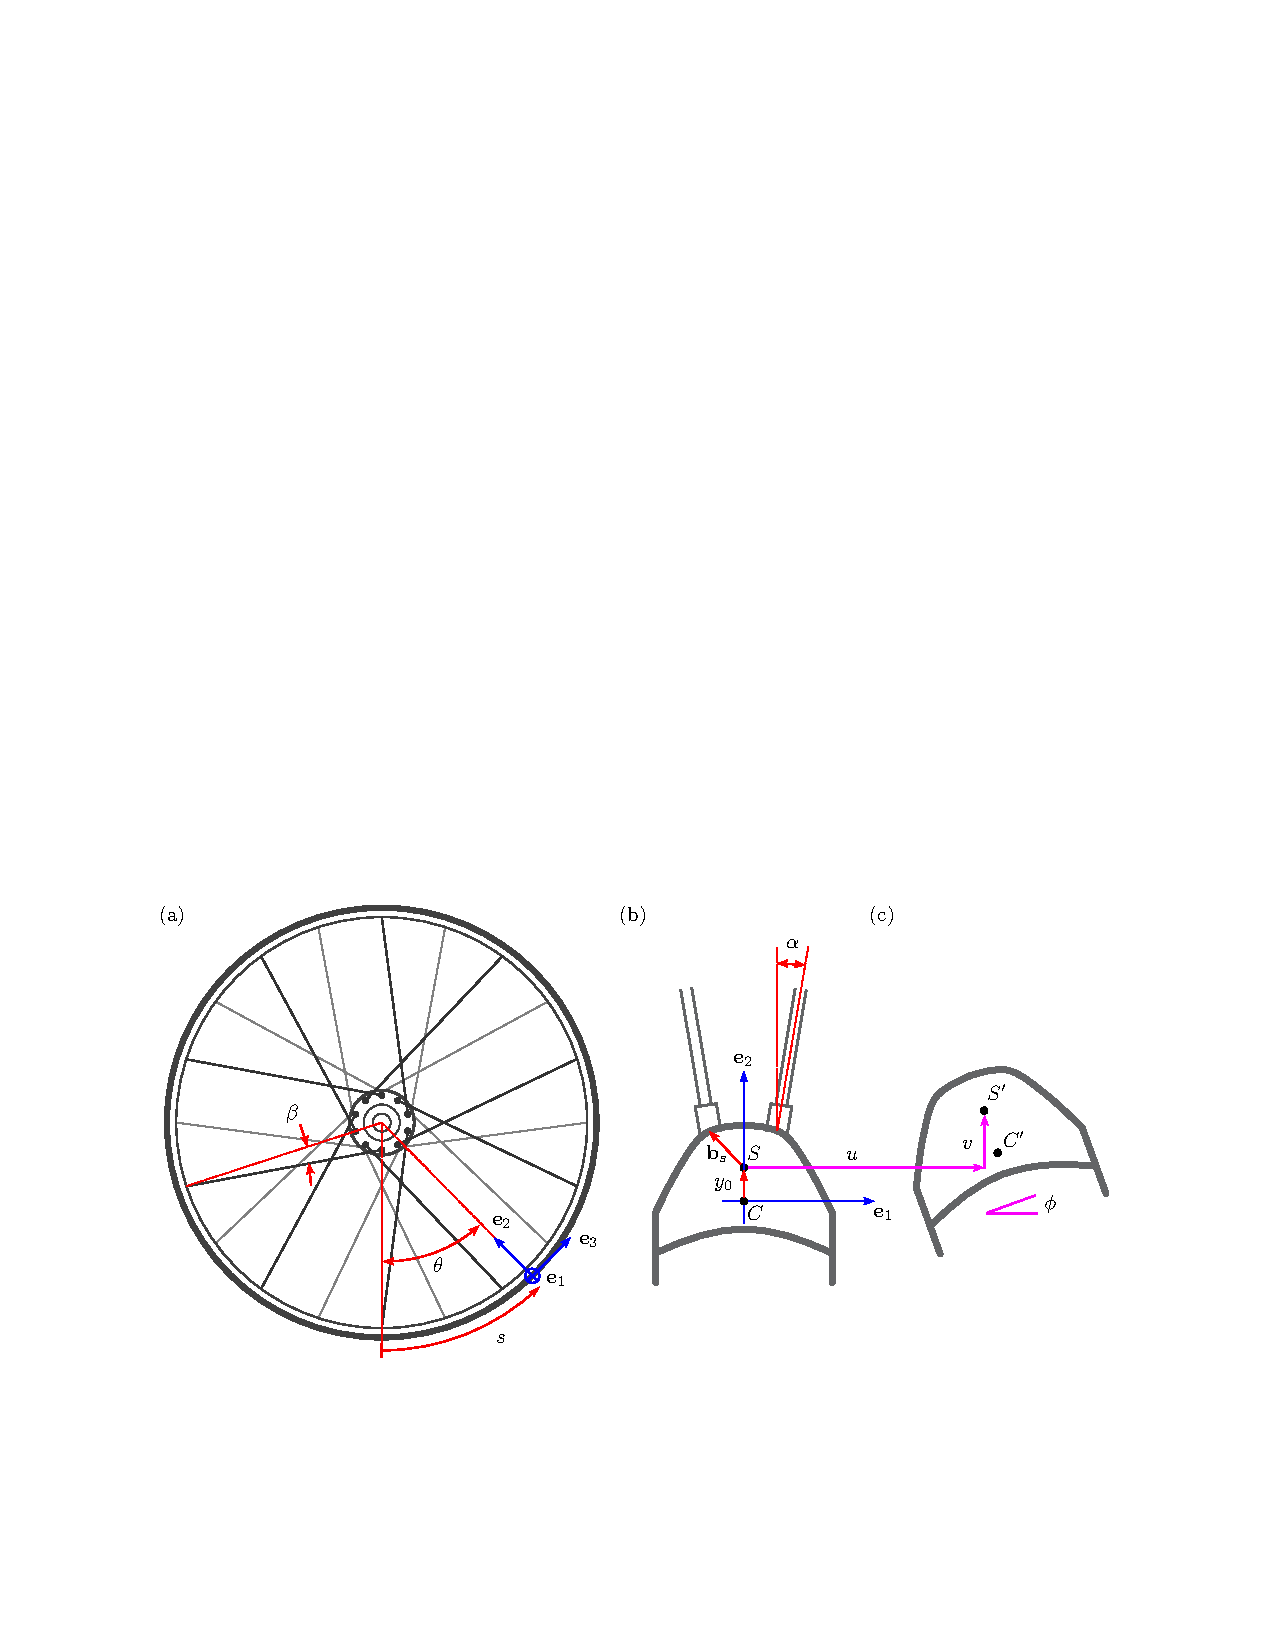
\includegraphics[width=4.0in]{fig_geometry.pdf}
    \end{center}
    \begin{block}{}
    {\tiny Image credit: Ford, Matthew, \emph{Reinventing the Wheel: Stress Analysis, Stability, and Optimization of the Bicycle Wheel}, PhD. Dissertation Northwestern University, December 2018.}
    \end{block}
\end{frame}

\begin{frame}{Wheel Truing}
	\begin{itemize}
        \item Spoke tension is adjusted by changing the effective length of the spoke via a threaded nipple seated in the rim
        \item Spoke tension consists of lateral, radial, and tangential components at the rim           
        \item Spoke tension is adjusted such that rim is `true' in both lateral and radial dimensions, and desired mean tension is achieved
        \item Conventional truing algorithm:
        \begin{enumerate}
            \item Adjust mean tension
            \item Minimize lateral variations
            \item Minimize radial variations
            \item Repeat until all desired specifications are met
        \end{enumerate}
	\end{itemize}
\end{frame}

\section{Apparatus}
  \begin{frame}{Apparatus}
    \begin{columns}[T] 
    \begin{column}[T]{5cm} 
        \begin{itemize}
        \item Centrimaster Comfort Wheel Truing Stand
        \item WheelFanatyk Digital Tension Gauge
        \item Canon EOS M, prime 22mm lens
        \item Wheel:  Stans ZTR Alpha Rim, DT Swiss Competition spokes, White Industries MI5 hub
        \end{itemize}
 \end{column}
 \begin{column}[T]{5cm} % alternative top-align that's better for graphics
      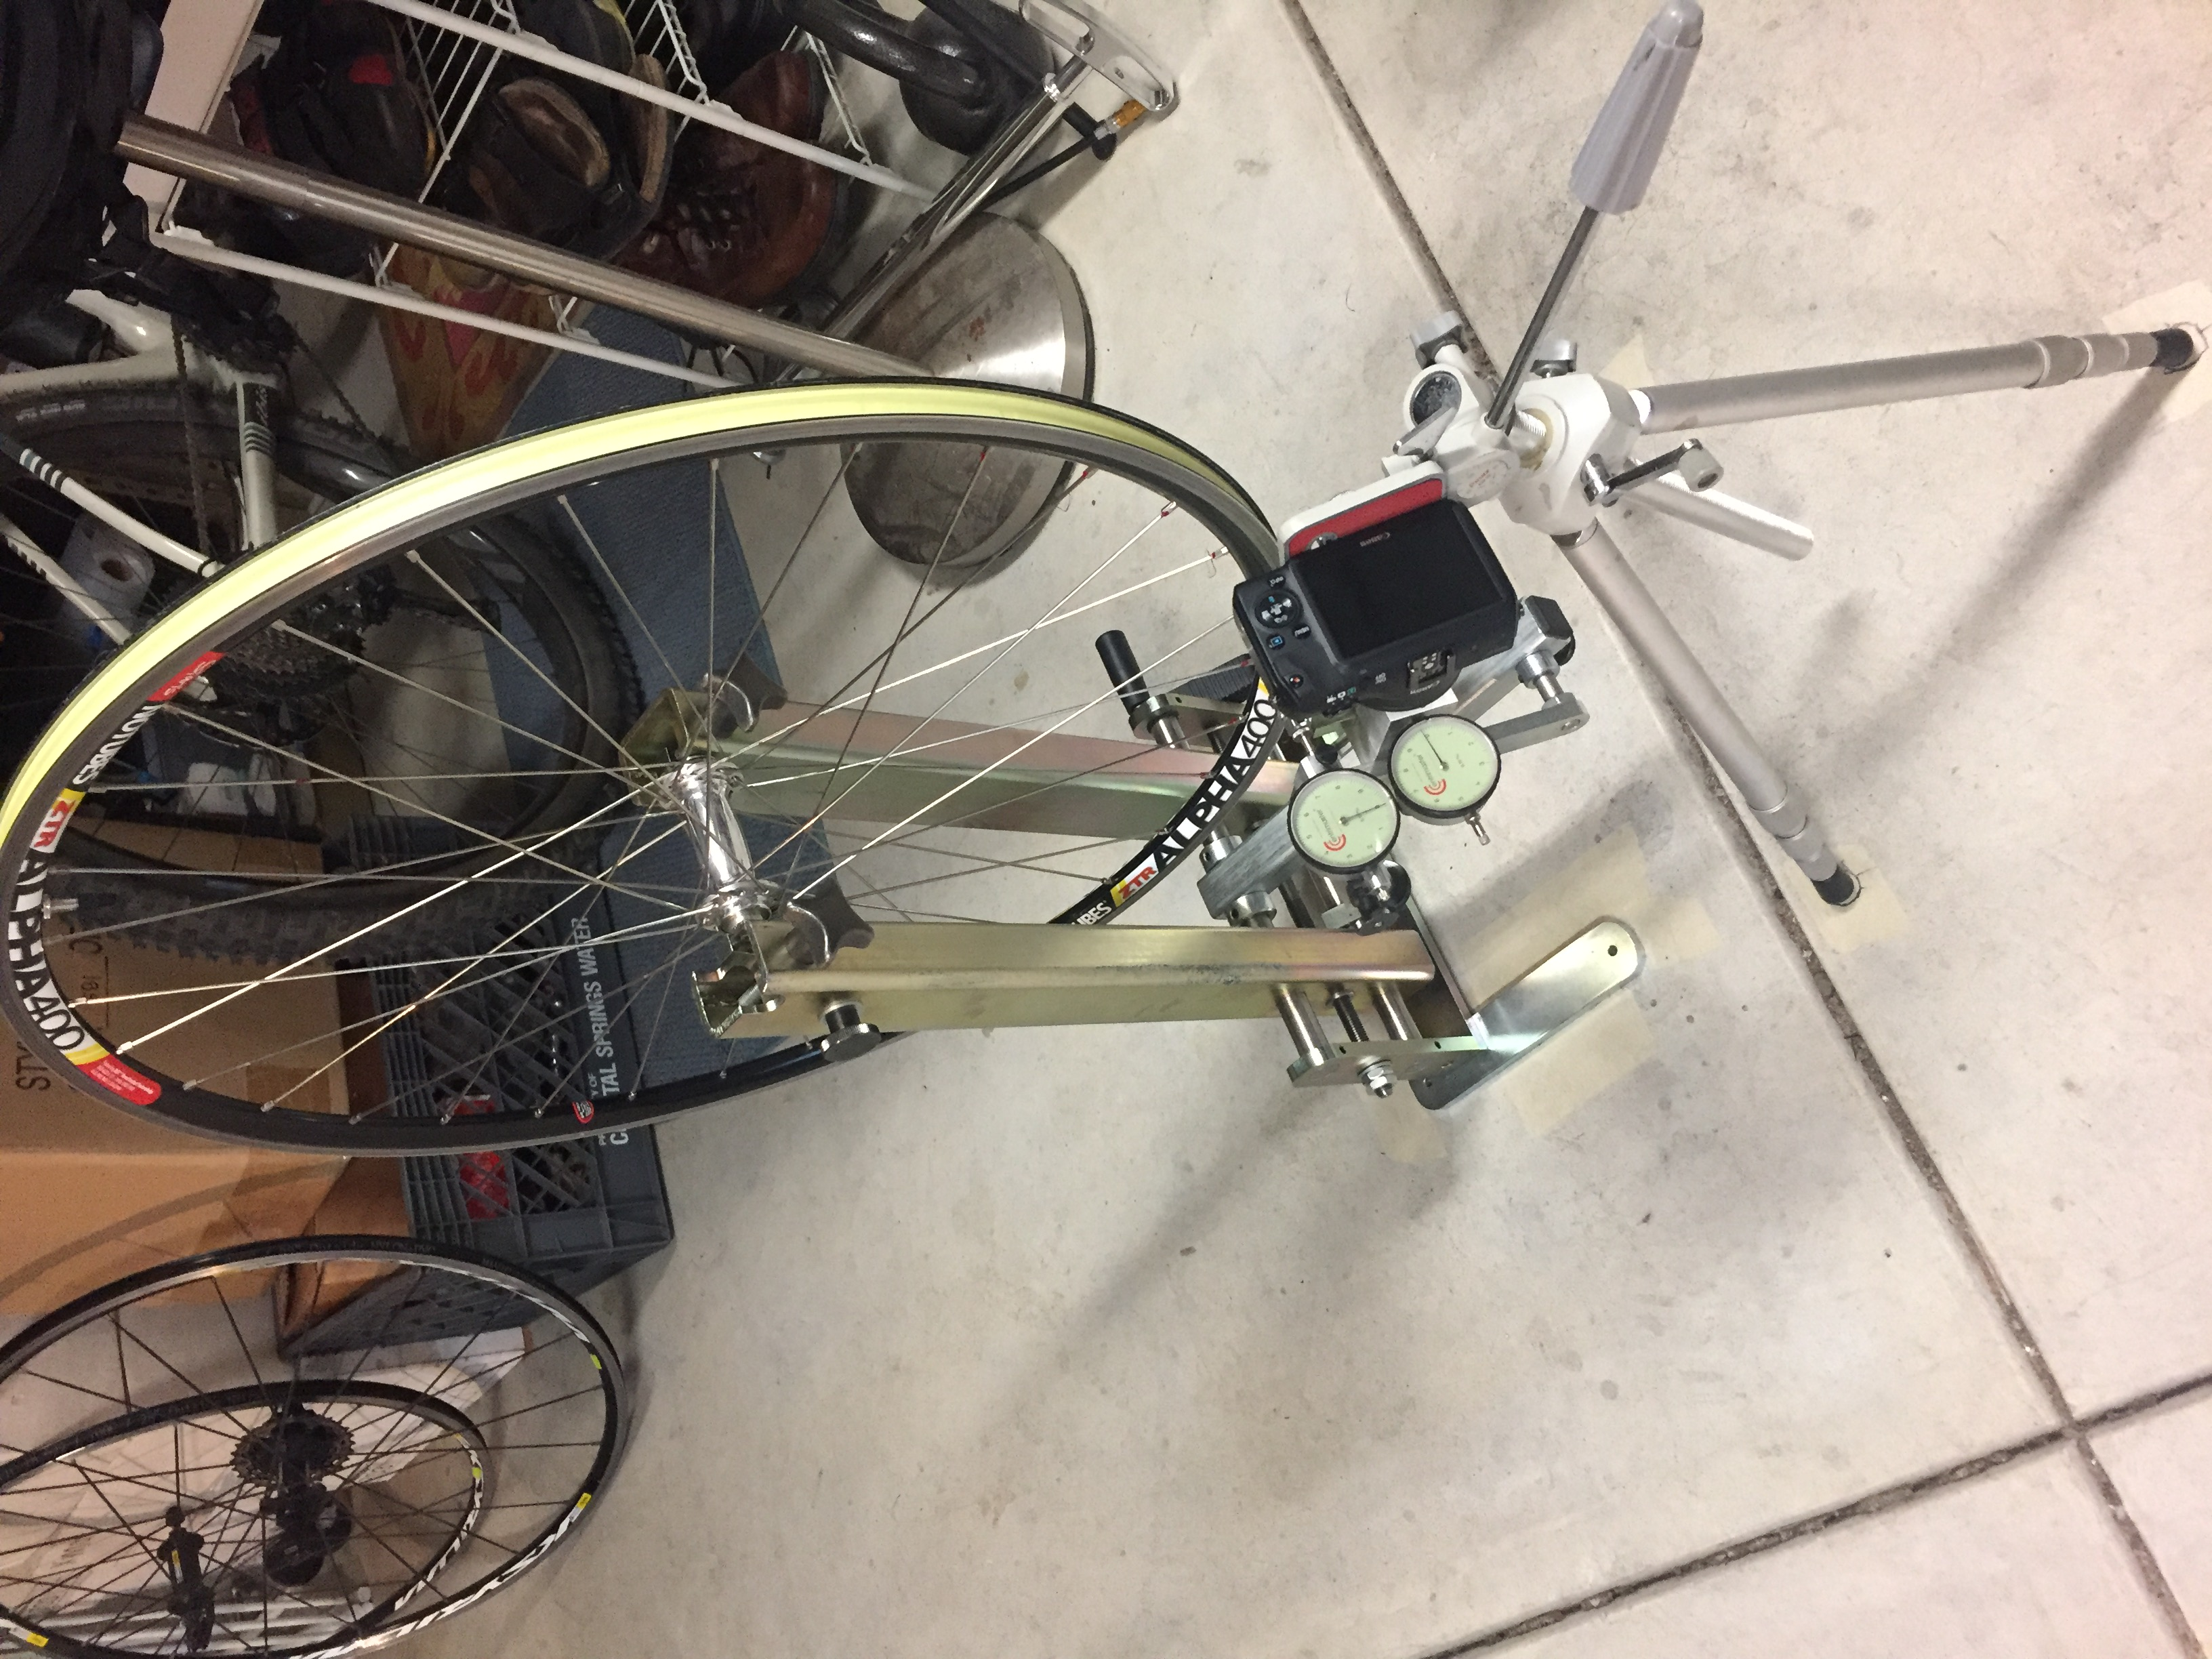
\includegraphics[totalheight=5cm, angle=-90]{apparatus}\\
     % 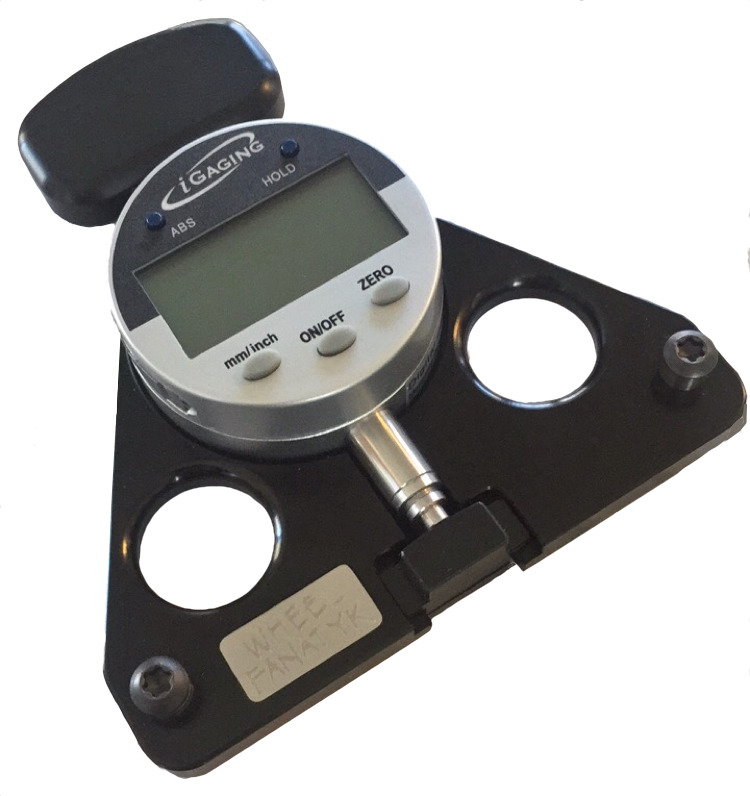
\includegraphics[height=3cm]{wheelfanatyk.jpg}
 \end{column}
 \end{columns}
  \end{frame}
  
\section{Method}
 
\begin{frame}
  \frametitle{System Identification Methodology}
  \centering
  \begin{block}{}
  Identify the lateral, radial and tension changes (`gain curves') induced by a unit spoke adjustment for each spoke
  \end{block}
  	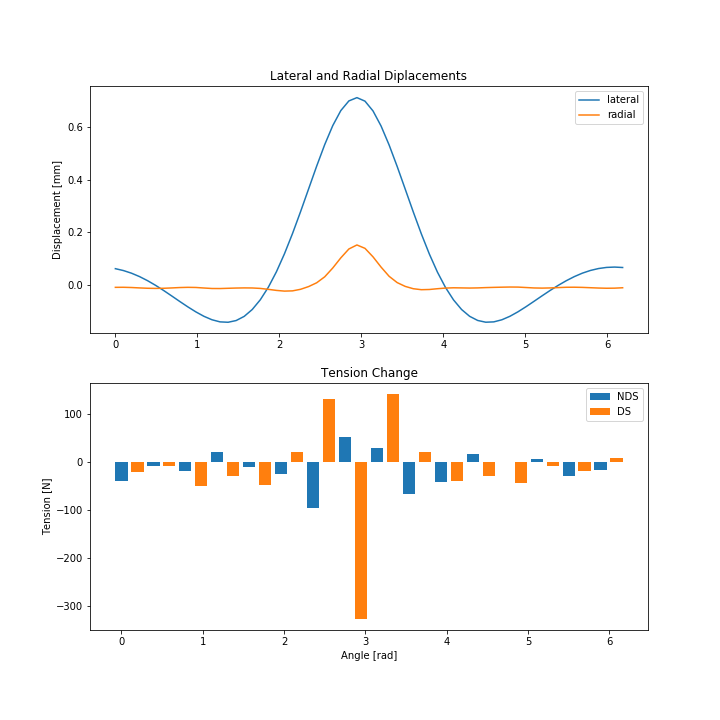
\includegraphics[height=2.3in]{GainCurveTheory}\\
	{\tiny Theoretical gain curves derived for a generic wheel using https://github.com/dashdotrobot/bike-wheel-calc}
\end{frame}

\begin{frame}
    \frametitle{Measurements Using Computer Vision}
    \begin{figure}
        \centering
        \begin{subfigure}[b]{0.2\textwidth}
            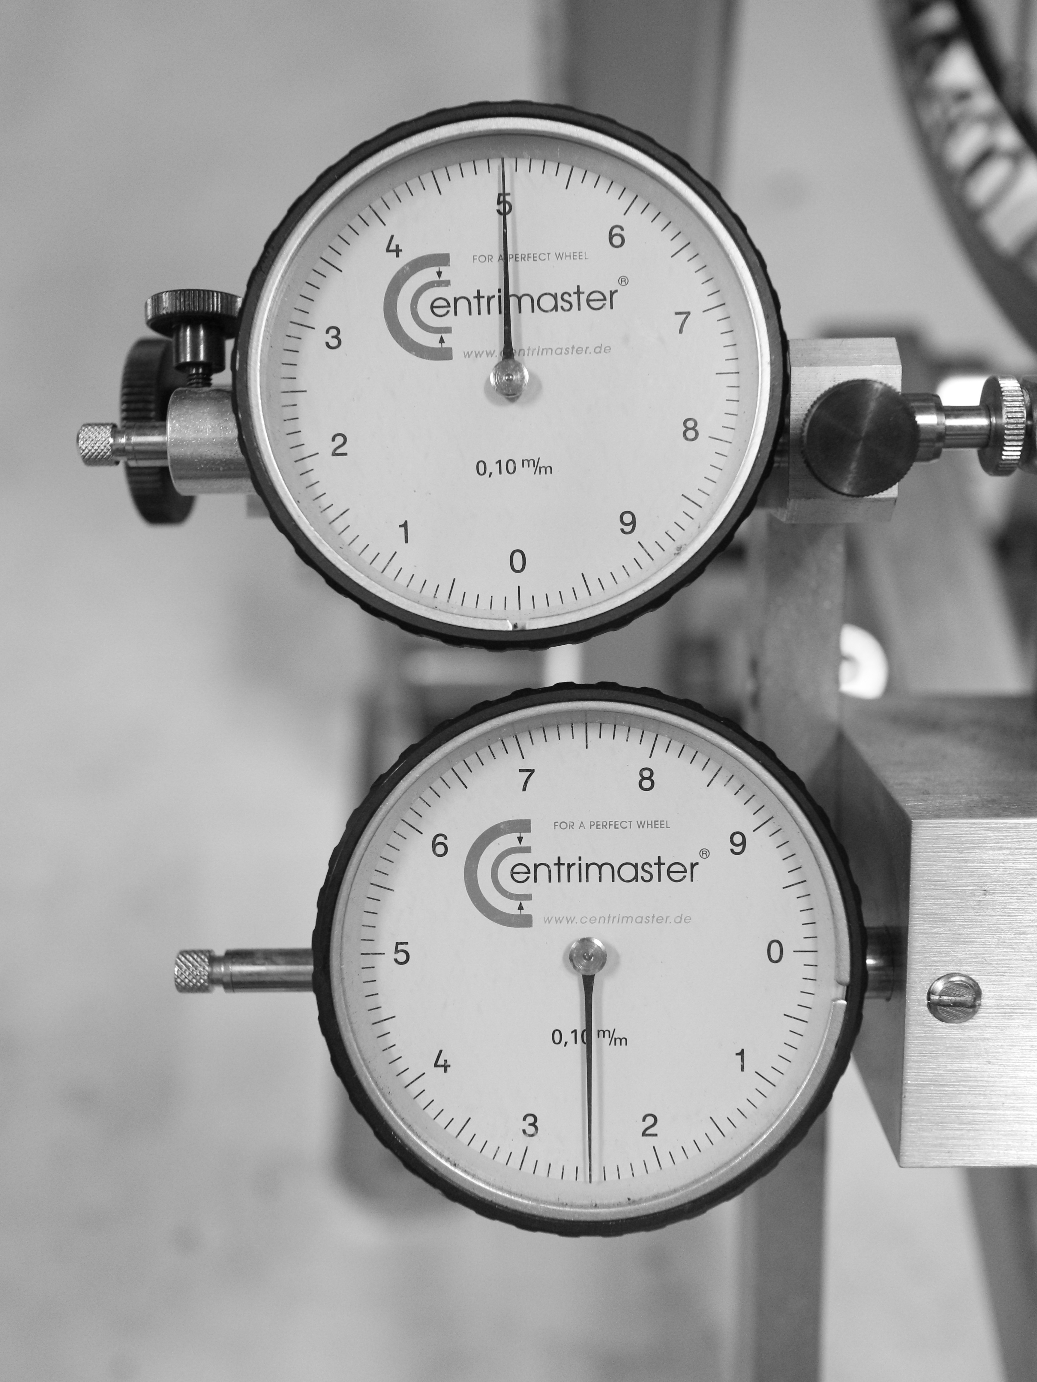
\includegraphics[width=\textwidth]{ref}
            \caption{}
        \end{subfigure}
         \quad %add desired spacing between images, e. g. ~, \quad, \qquad, \hfill etc. 
          %(or a blank line to force the subfigure onto a new line)
        \begin{subfigure}[b]{0.2\textwidth}
            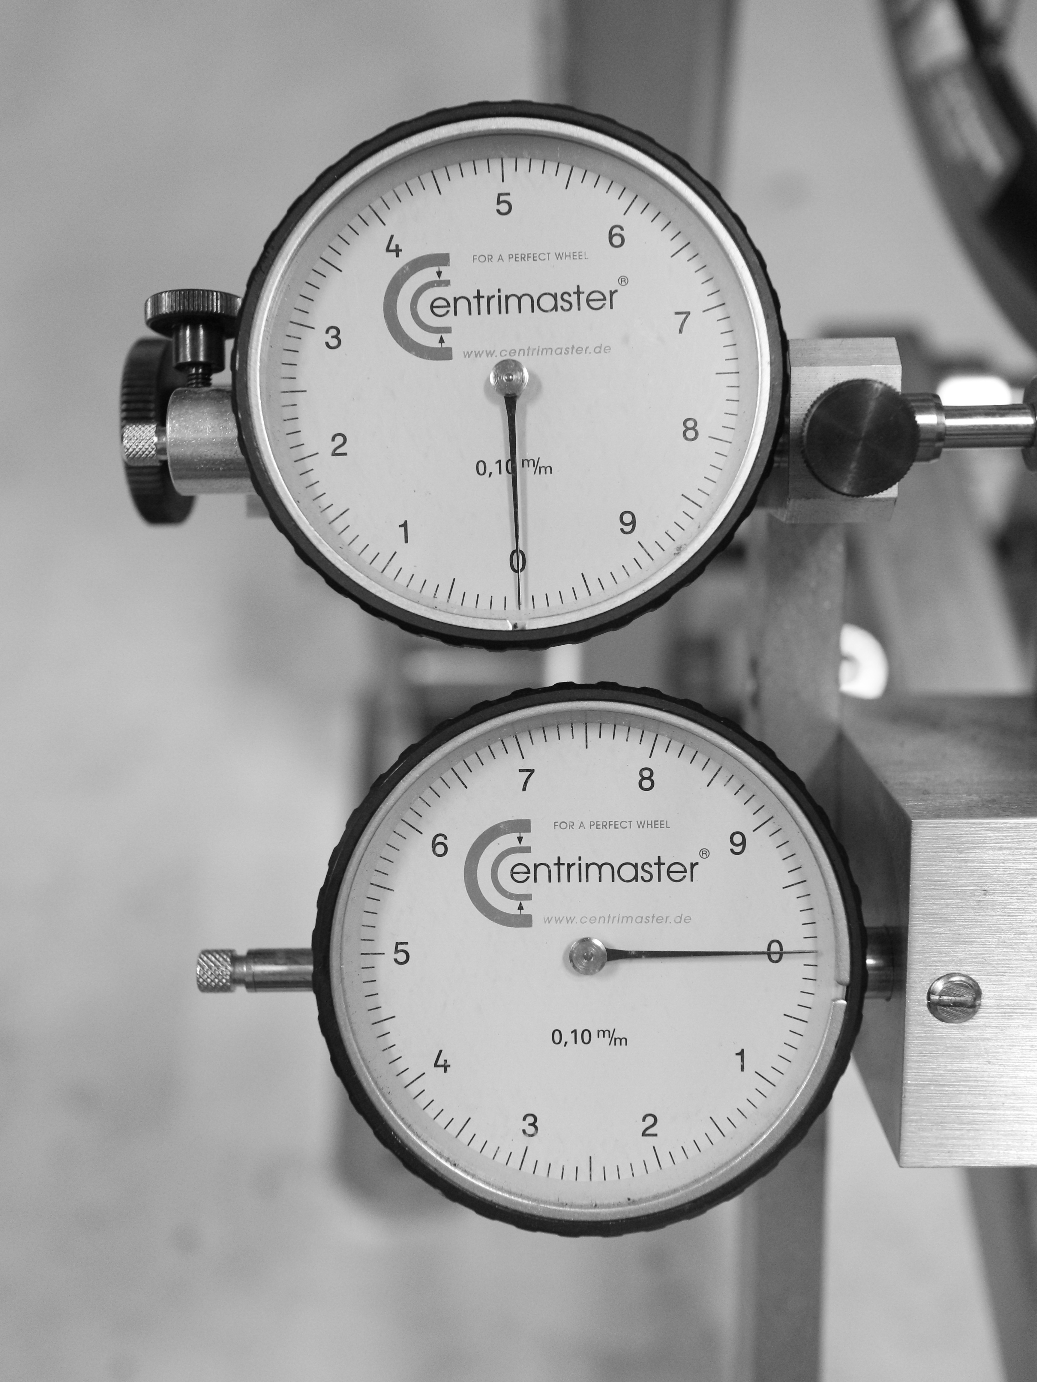
\includegraphics[width=\textwidth]{zero}
            \caption{}
        \end{subfigure}
        \quad
        \begin{subfigure}[b]{0.2\textwidth}
            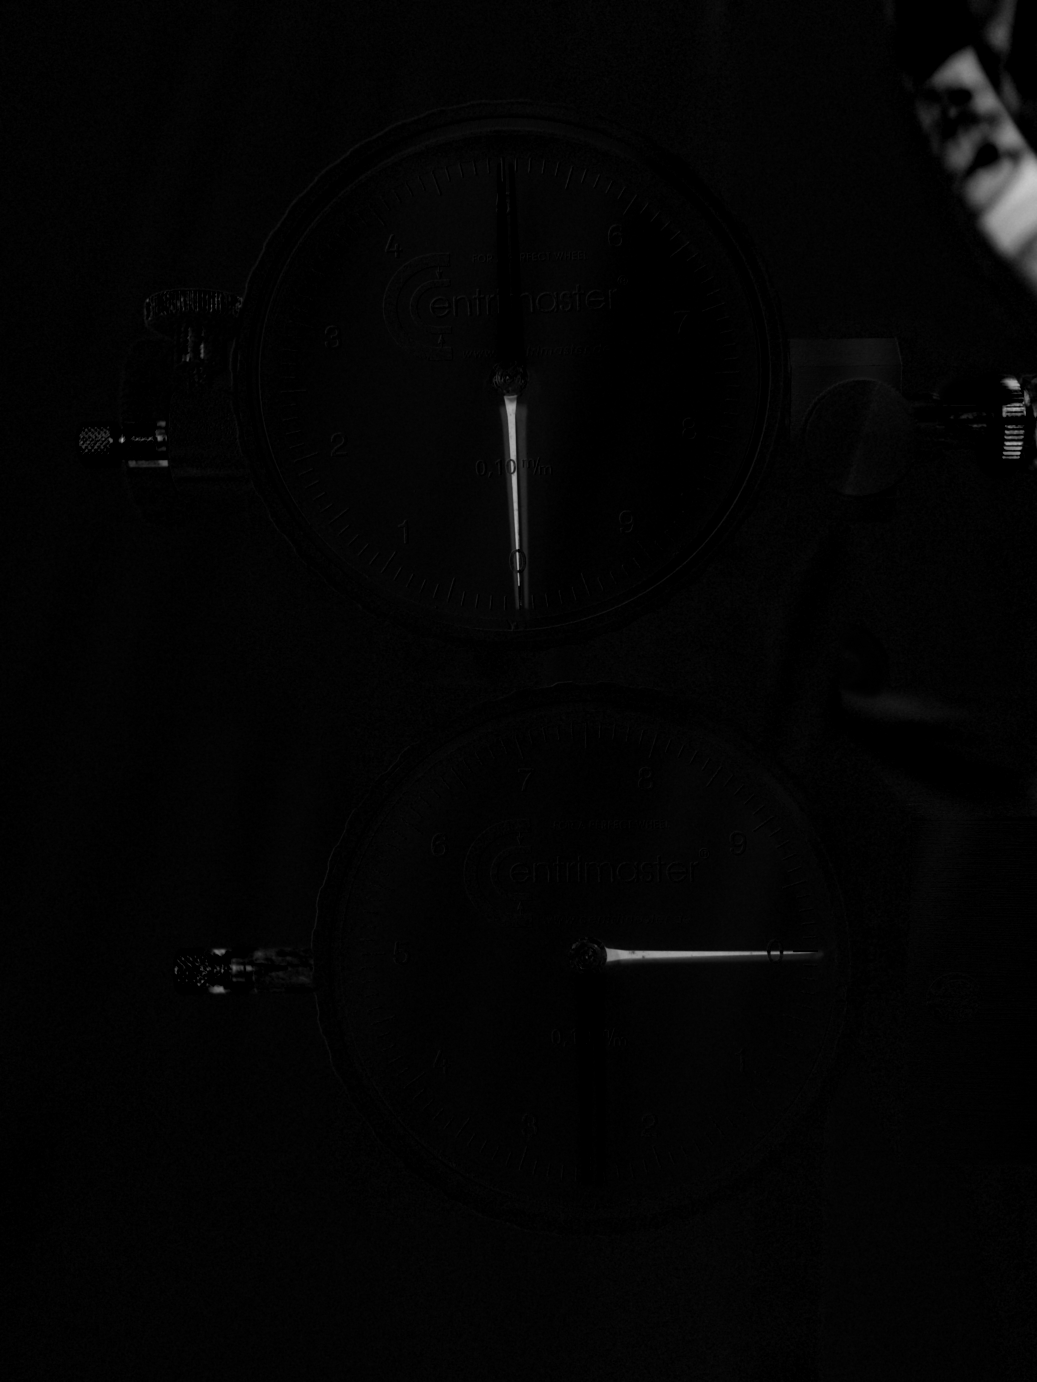
\includegraphics[width=\textwidth]{delta_img}
            \caption{}
        \end{subfigure}
         \quad
        \begin{subfigure}[b]{0.2\textwidth}
            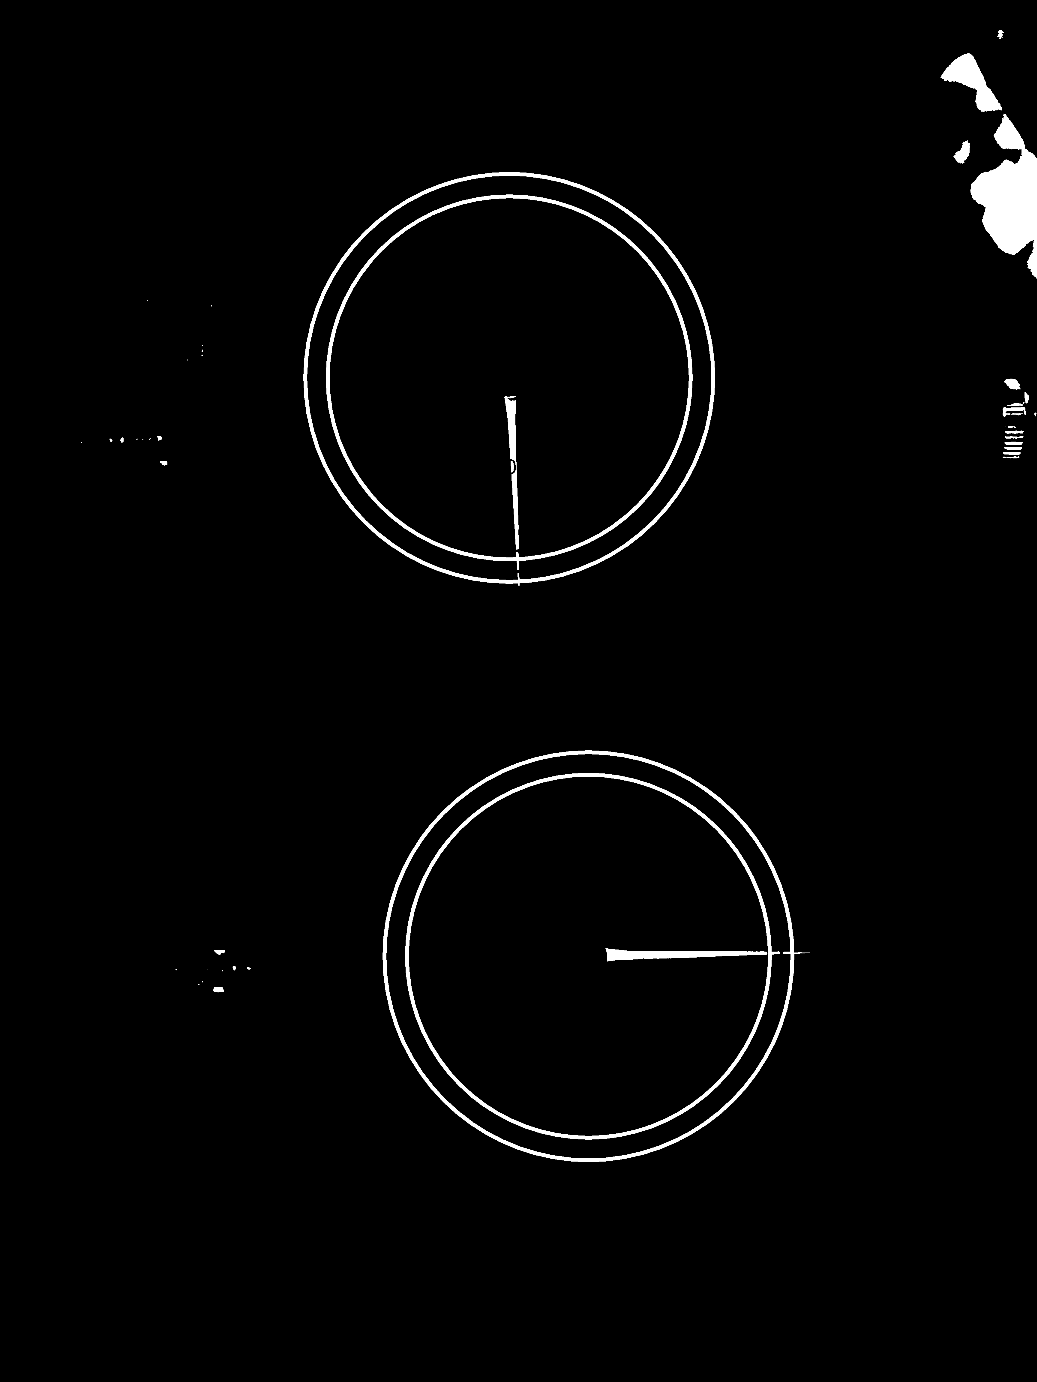
\includegraphics[width=\textwidth]{threshold_img}
            \caption{}
        \end{subfigure}
    \end{figure}
    Algorithm to interpret gauge displacements:
        \begin{enumerate}
            \item Reference image (a)
            \item Measurement (or zero value) image (b)
            \item Subtract measurement from reference (c) 
            \item Binary threshold and mask (d)
            \item Calculate angle of centroid from gauge center
            \item Calculate displacement measurement from angle
        \end{enumerate}
\end{frame}

\begin{frame}
      \frametitle{Spoke Tension Measurements}
      \begin{figure}
      	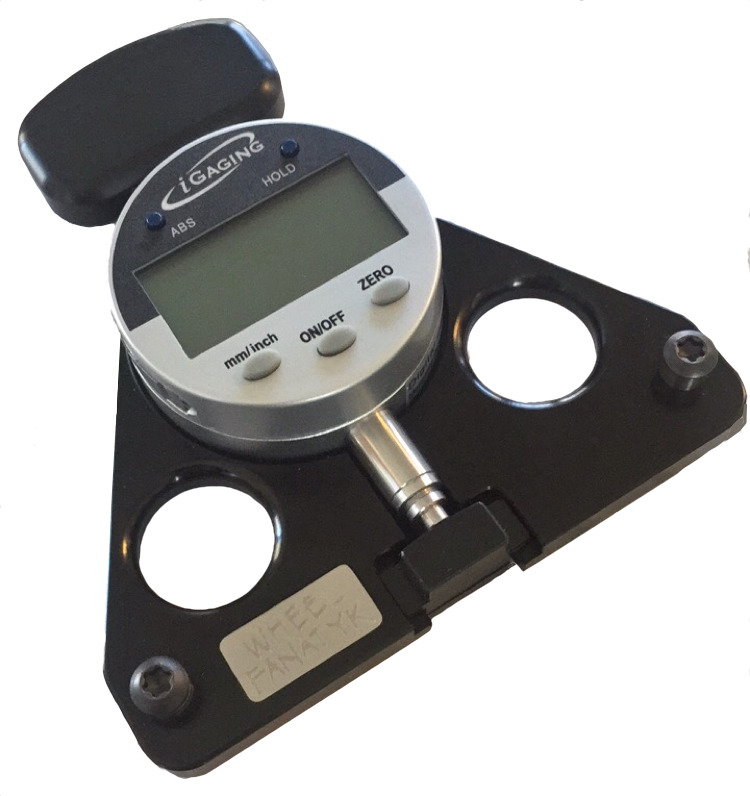
\includegraphics[height = 2.5cm]{wheelfanatyk}\\
        {\tiny WheelFanatyk spoke tension meter.  Image credit: https://www.wheelfanatyk.com}
      \end{figure}

      \begin{itemize}
          \item Digital spoke tension measurements
          \item Data collected through USB to PC
          \item Meter collects displacement of spoke by calibrated spring
          \item Reference measurement accounts for variation of spoke thickness 
          \item Tension values interpolated from calibration table
      \end{itemize}•
\end{frame}

\begin{frame}
\frametitle{Measurement Data Vector}
Measurement data collected for a wheel under test:
\begin{align*}
    \bf U &=  \begin{bmatrix}
        u(\theta = 1\frac{2\pi}{2n_s})\\
        u(\theta = 2\frac{2\pi}{2n_s})\\
        \vdots\\
        u(\theta = 2n_s\frac{2\pi}{2n_s})
        \end{bmatrix}
    \bf V = \begin{bmatrix}
        v(\theta = 1\frac{2\pi}{2n_s})\\
        v(\theta = 2\frac{2\pi}{2n_s})\\
        \vdots\\
        v(\theta = 2n_s\frac{2\pi}{2n_s})
    \end{bmatrix}
        \bf T = \begin{bmatrix}
        t(\theta = 1\frac{2\pi}{n_s})\\
        t(\theta = 2\frac{2\pi}{n_s})\\
        \vdots\\
        t(\theta = n_s\frac{2\pi}{n_s})
    \end{bmatrix} \\
    \bf Y &= \begin{bmatrix}
    \bf U\\\bf V\\ \bf T
    \end{bmatrix}
    \end{align*}
\begin{itemize}
    \item $n_s$ = number of spokes
    \item $\theta=$ rim measurement location where $\theta = 0$ is taken to be the valve hole
    \item $u(\theta)=$ lateral measurement at $\theta$
    \item $v(\theta) = $ radial measurement at $\theta$
    \item $t(\theta)=$ spoke tension measurement at $\theta$
\end{itemize}
\end{frame}

\begin{frame}
\frametitle{Gain Matrices}
Let $\bf{u_s}$=$u_s(\theta)$ be the lateral displacement vector (gain curve) for every discrete $\theta$ around the rim induced by turning spoke $s$ by one rotation.  The matrix of all $\bf u_s$ gain curves is defined to be the lateral `gain' matrix $\Phi_u$.  The radial and tension gain matrices are similarly defined.
\begin{align*}
     \Phi_u &= \begin{bmatrix}
     \bf u_1 & \bf u_2& \dots & \bf u_{n_s}
     \end{bmatrix}\\
     \Phi_v &= \begin{bmatrix}
     \bf v_1 & \bf v_2& \dots & \bf v_{n_s}
     \end{bmatrix}\\     
     \Phi_t &= \begin{bmatrix}
     \bf t_1 & \bf t_2& \dots & \bf t_{n_s}
     \end{bmatrix} 
     \end{align*}
\end{frame}

\begin{frame}
\frametitle{Measurement Prediction}
Let $\bf d$ be a vector of spoke rotations. Let $\bf Y_b$ be the baseline wheel measurements, that is, the state of the wheel prior to the application of $\bf d$. The predicted lateral, radial, and tension measurements, $\bf \hat Y$, after applying $\bf d$ to the spokes is given by:
\begin{align*}
    \Phi &= \begin{bmatrix}
        \Phi_u\\
        \Phi_v\\
        \Phi_t
    \end{bmatrix}\\
   \bf \hat Y&= {\bf Y_b} + \Phi \bf d\\
\end{align*}
\end{frame}

\begin{frame}
\frametitle{Multi-objective Least Squares}
Predict the set of spoke rotations, $\bf \hat d$, that yield given set of measurements, $\bf Y$ given the weighting factors $\mu_v$, $\mu_t$ and desired state $\bf Y_d = [\bf u_d, v_d, T_d]^T$:
    \begin{align*}
    \tilde \Phi &= \begin{bmatrix}
    \Phi_u\\
    \Phi_v \sqrt {\mu_v}\\
    \Phi_t \sqrt {\mu_t}
    \end{bmatrix}
     \Delta \bf \tilde Y = \begin{bmatrix}
    \bf u - u_d \\
   ( {\bf v - v_d} )  \sqrt {\mu_v}\\
    ( {\bf  T - T_d} )  \sqrt {\mu_t}
    \end{bmatrix}  \\
        {\bf \hat d} &= \tilde \Phi^\dagger \Delta {\bf \tilde Y}
    \end{align*}
	Where $\tilde \Phi^\dagger$ is the pseudo-inverse of $\tilde \Phi$.  The weighting factors represent the tradeoff between the lateral, radial, and tension variables and are found through evaluation of the wheel specification and exhaustive simulation.
\end{frame}

\begin{frame}
        \frametitle{Truing Algorithm}
        \begin{itemize}
          \item $\bf \hat d$ is the best fit of spoke rotations that result in the measured state relative to the desired state
          \item To achieve the desired state therefore apply $-\bf \hat d$ to the system
          \item Spoke turns are difficult to apply accurately.  Instead predict the state of the system after each spoke adjustment (element of $-\bf \hat d$)
          \item Adjust the spoke until the lateral displacement at the spoke location matches the prediction
          \item After all spokes adjusted, measure state of the system
          \item Demonstrated graphically in the next slide...
        \end{itemize}
\end{frame}

\begin{frame}
\frametitle{Truing Algorithm}
\begin{figure}
    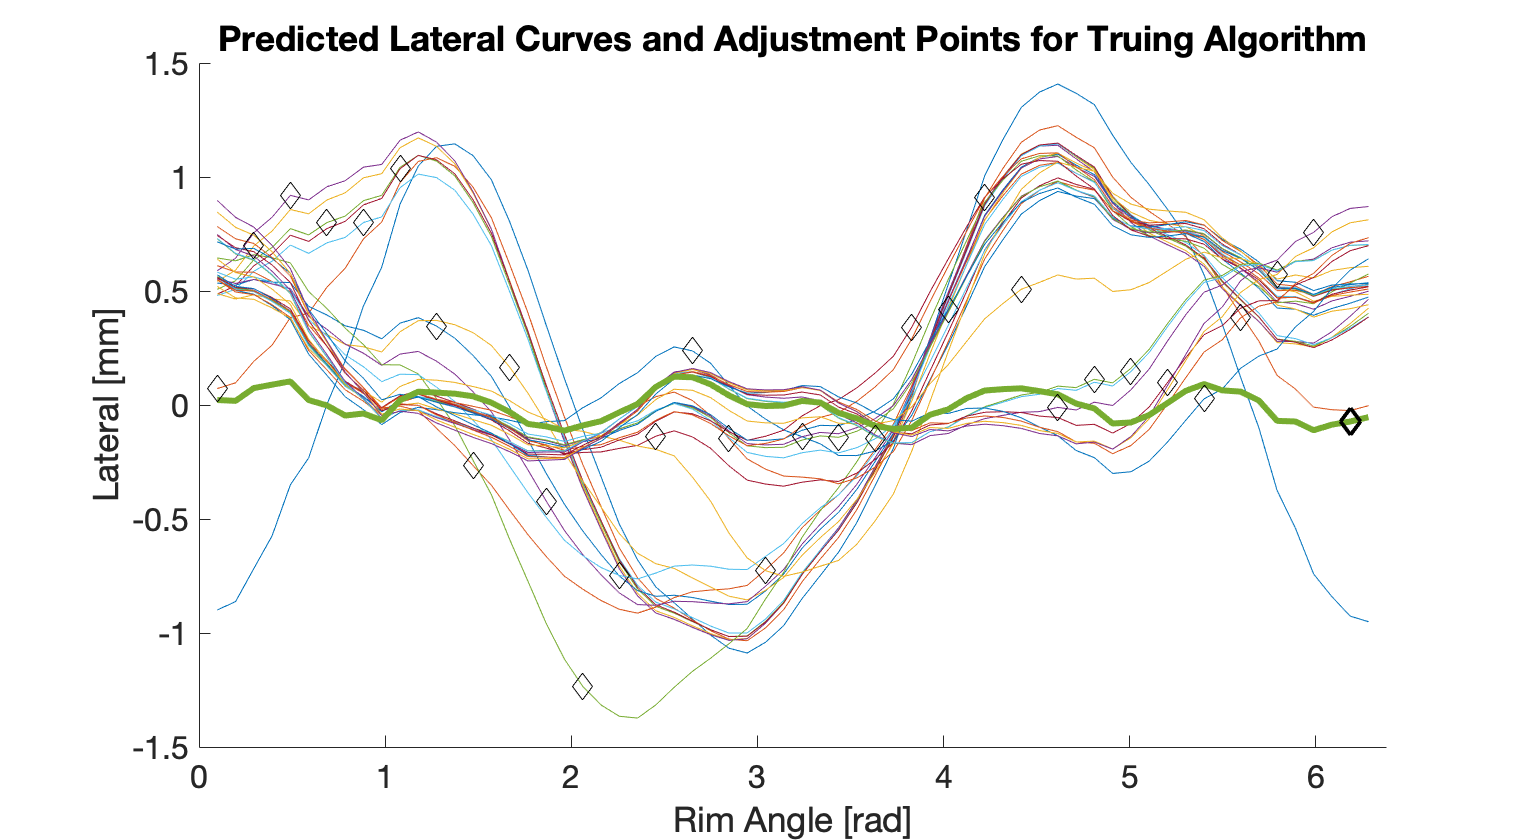
\includegraphics[width=0.9\textwidth]{algorithm}
\end{figure}
{The predicted lateral profiles after each spoke adjustment during truing.  The diamonds are the lateral target points at the spoke being adjusted.  The blue curve represents the profile \emph{after} the first spoke adjustment, the green curve represents the final (trued) profile.}
\end{frame}

\section{Results}

\begin{frame}
\frametitle{Computer Vision Validation}
    \begin{figure}
    	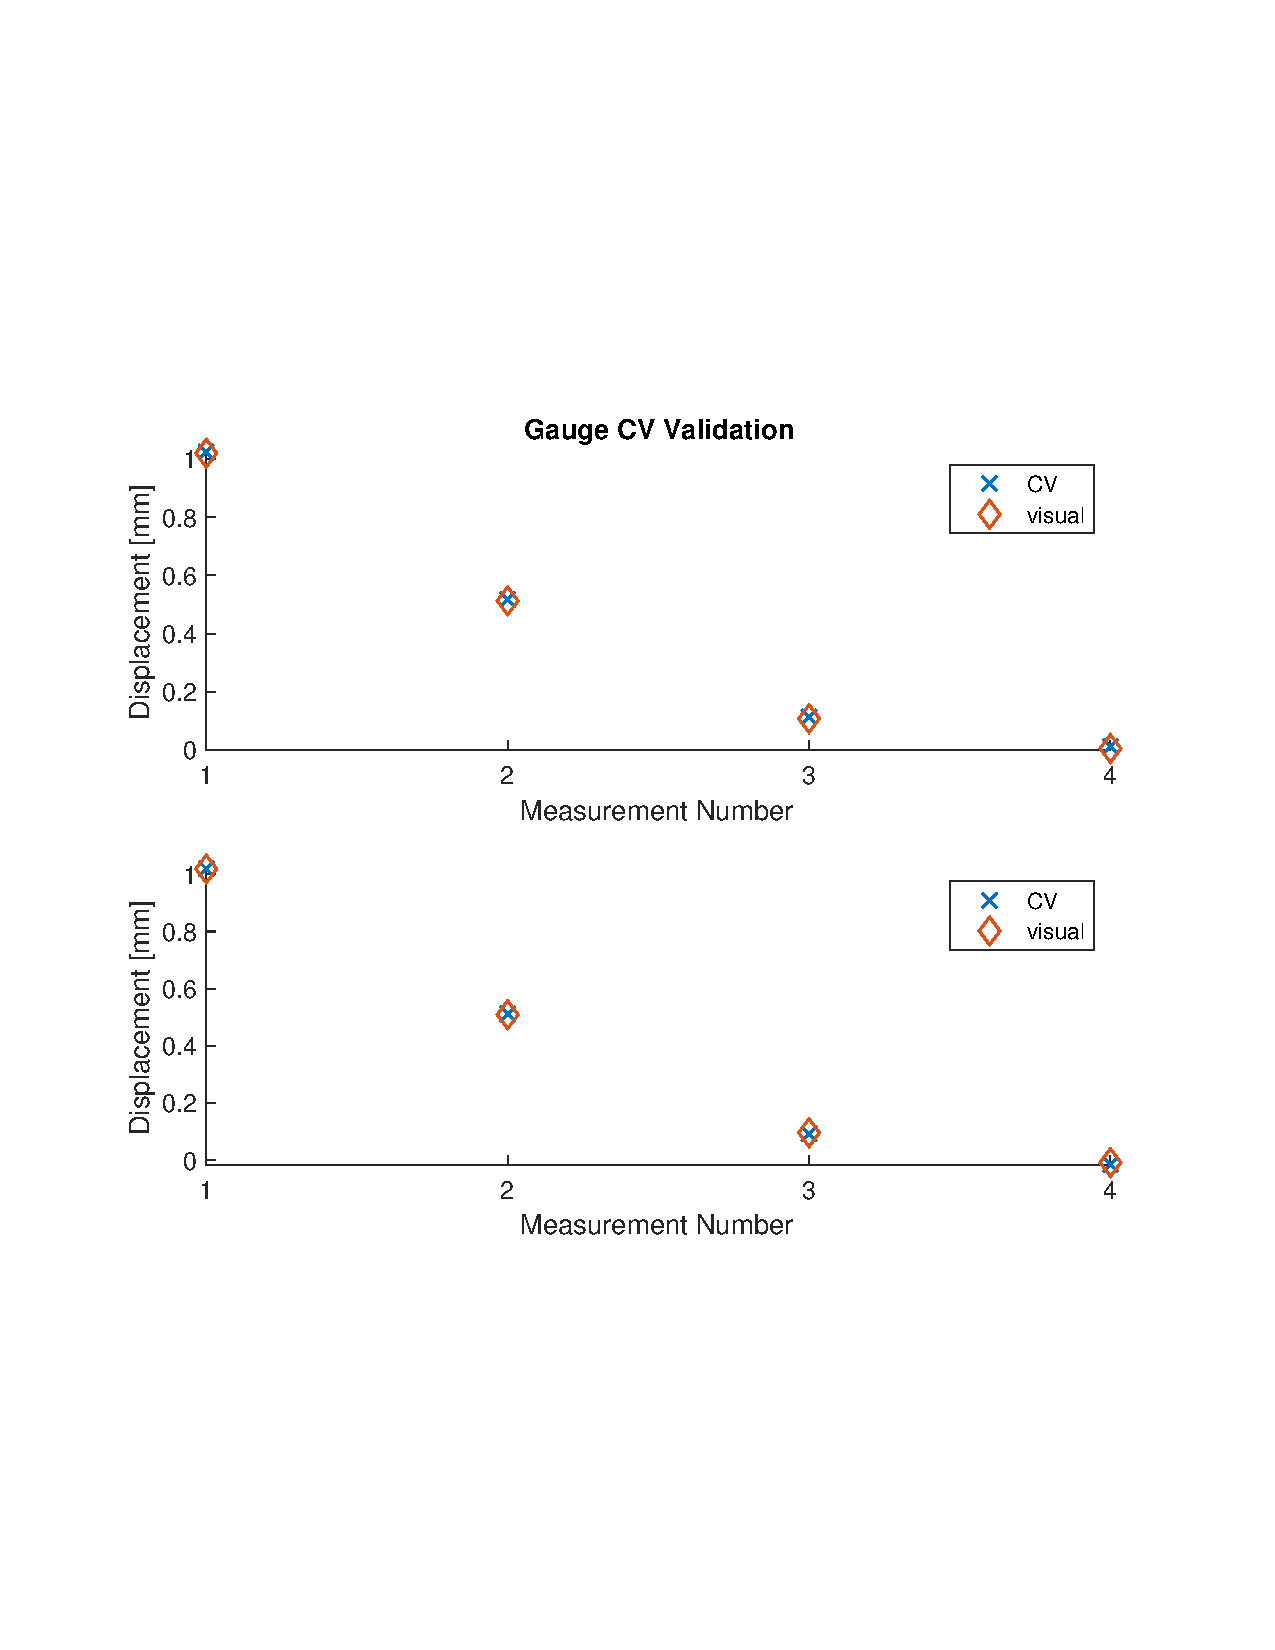
\includegraphics[width=7cm,trim=0 200 0 200]{gaugeCV_validation}
    \end{figure}
    \begin{itemize}
    \item Four dual gauge readings were recorded
    \item Gauges were set to 1mm, 0.5mm, 0.1mm, and 0mm
    \item Visual analysis and CV algorithm results compared
    \item  Visual analysis resolution is 0.0135mm
    \item Results agree to $\pm$ 0.007mm
    \end{itemize}
\end{frame}

\begin{frame}
\frametitle{Tension Gain Curves}
\begin{columns}[T] 
    \begin{column}[T]{5.25cm} 
        \begin{itemize}
        \item 32 tension curves were collected
        \item Four distinct patterns identified:
        	\begin{itemize}
            \item Non-drive side leading
            \item Drive side leading
            \item Non-drive side trailing
            \item Drive side trailing
	\end{itemize}
	\item Tension meter discretization leads to bias so average curve used for all spokes
        \end{itemize}
     \end{column}
     \begin{column}[T]{5cm} % alternative top-align that's better for graphics
          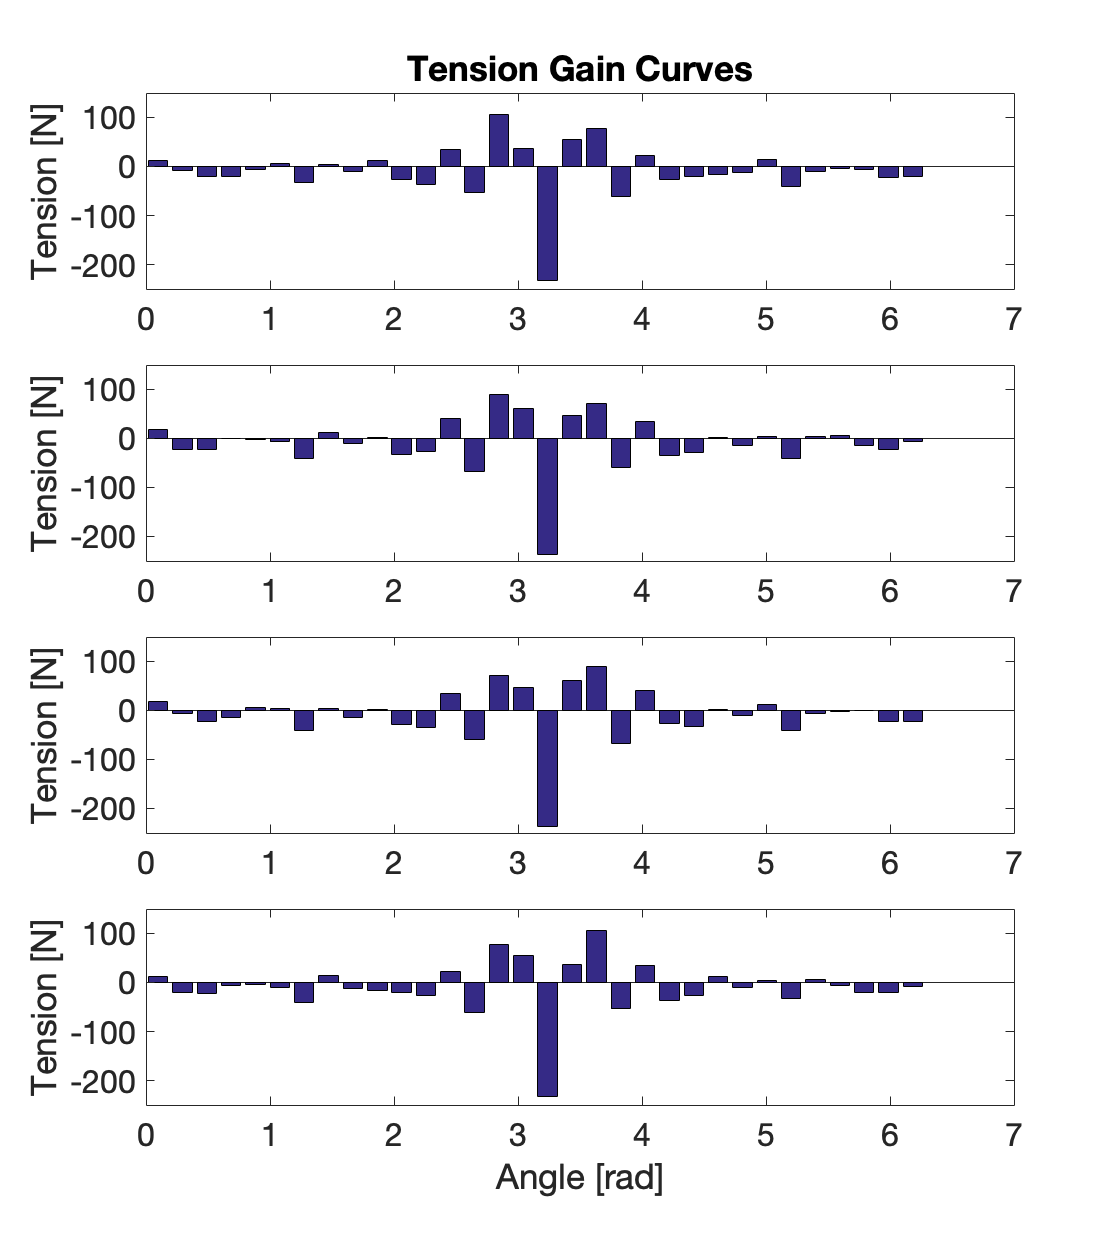
\includegraphics[totalheight=6cm]{TensionGC}
     \end{column}
 \end{columns}
\end{frame}

\begin{frame}
\frametitle{Lateral and Radial Gain Curves	}
\begin{figure}
        \centering
        \begin{subfigure}[b]{0.475\textwidth}
            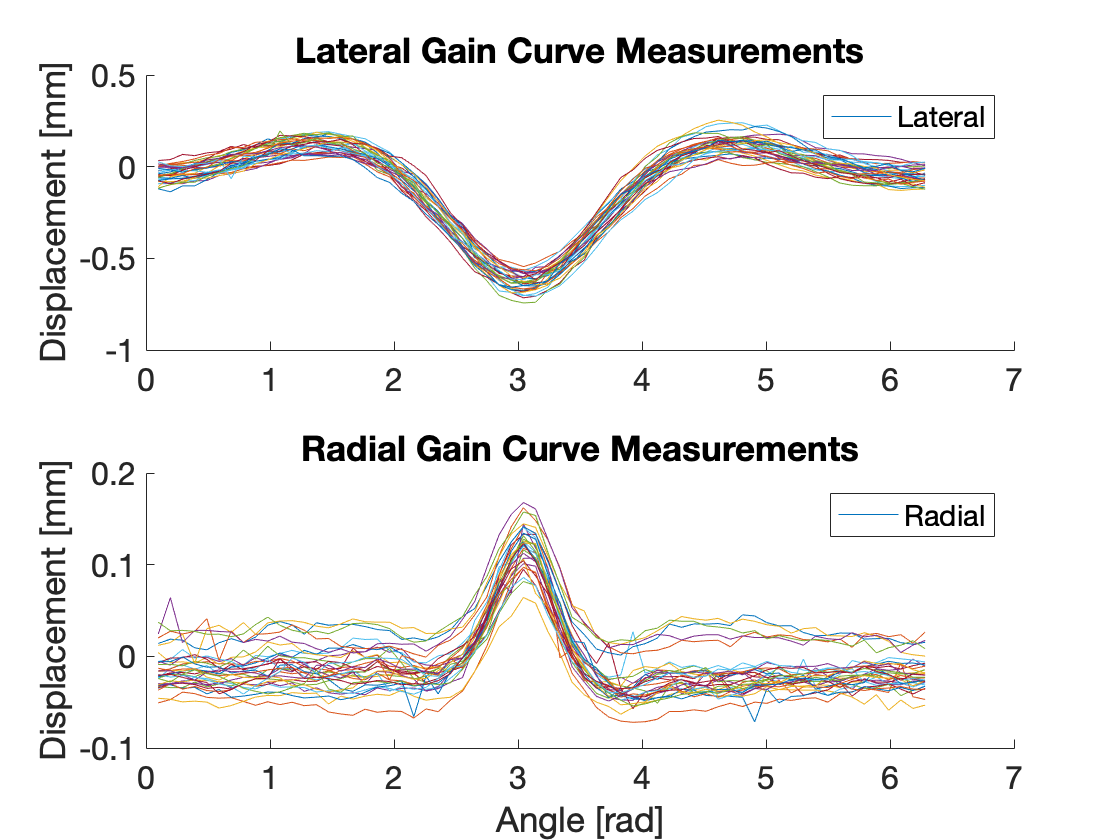
\includegraphics[width=\textwidth]{lat_rad_GC_raw}
            \caption{}
        \end{subfigure}
        \begin{subfigure}[b]{0.475\textwidth}
            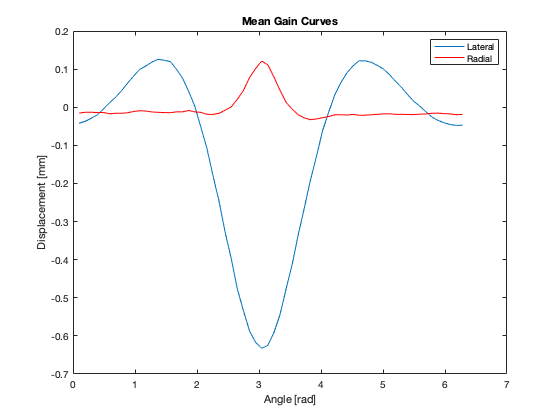
\includegraphics[width=\textwidth]{lat_rad_GC_mean}
            \caption{}
        \end{subfigure}
\end{figure}
\begin{itemize}
    \item 32 lateral and radial curves measured (a)
    \item Mean gain curves used for model (b)
    \item Curves normalized to same rim angle and side for clarity
\end{itemize}
\end{frame}

\begin{frame}
\frametitle{Truing Algorithm Simulation}
\begin{figure}
        \centering
        \begin{subfigure}[b]{0.45\textwidth}
            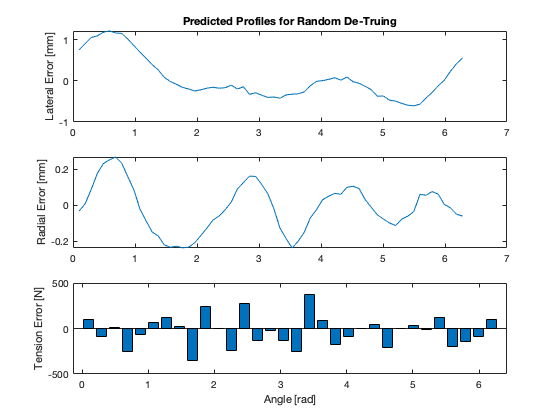
\includegraphics[width=\textwidth]{detune}
        \end{subfigure}
        ~
        \begin{subfigure}[b]{0.45\textwidth}
            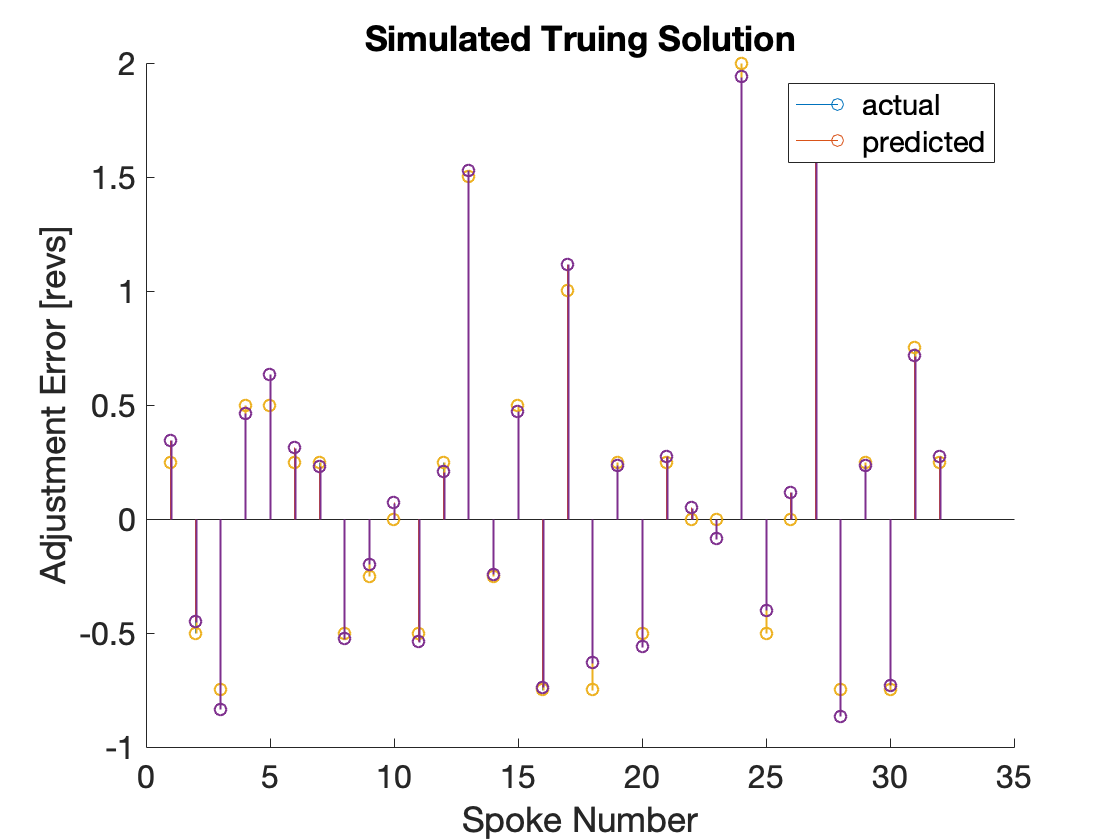
\includegraphics[width=\textwidth]{simtrue}
        \end{subfigure}
\end{figure}
\begin{itemize}
    \item Random spoke displacement vector, $\bf d$,  generated
    \item Noise added to simulated profile
    \item Spoke displacement vector, $\bf \hat d$, predicted
    \item Weighting factors adjusted for performance
\end{itemize}
\end{frame}

\begin{frame}
\frametitle{Simulation Error}
\begin{columns}[T]
    \begin{column}[T]{5cm}
    Weighting factors yielding satisfactory performance:
    \begin{itemize}
    \item $\mu_v = 0.5$
    \item $\mu_t = 1.0e-5$ 
    \end{itemize}
    \end{column}
    \begin{column}[T]{5cm} 
        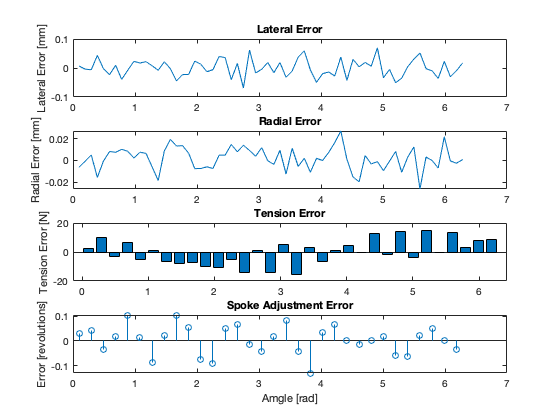
\includegraphics[width=\textwidth]{simerr}
    \end{column}
\end{columns}
\end{frame}

\begin{frame}
\frametitle{Experiment 1: De-true Test Wheel}
\begin{figure}
        \centering
        \begin{subfigure}[b]{0.45\textwidth}
            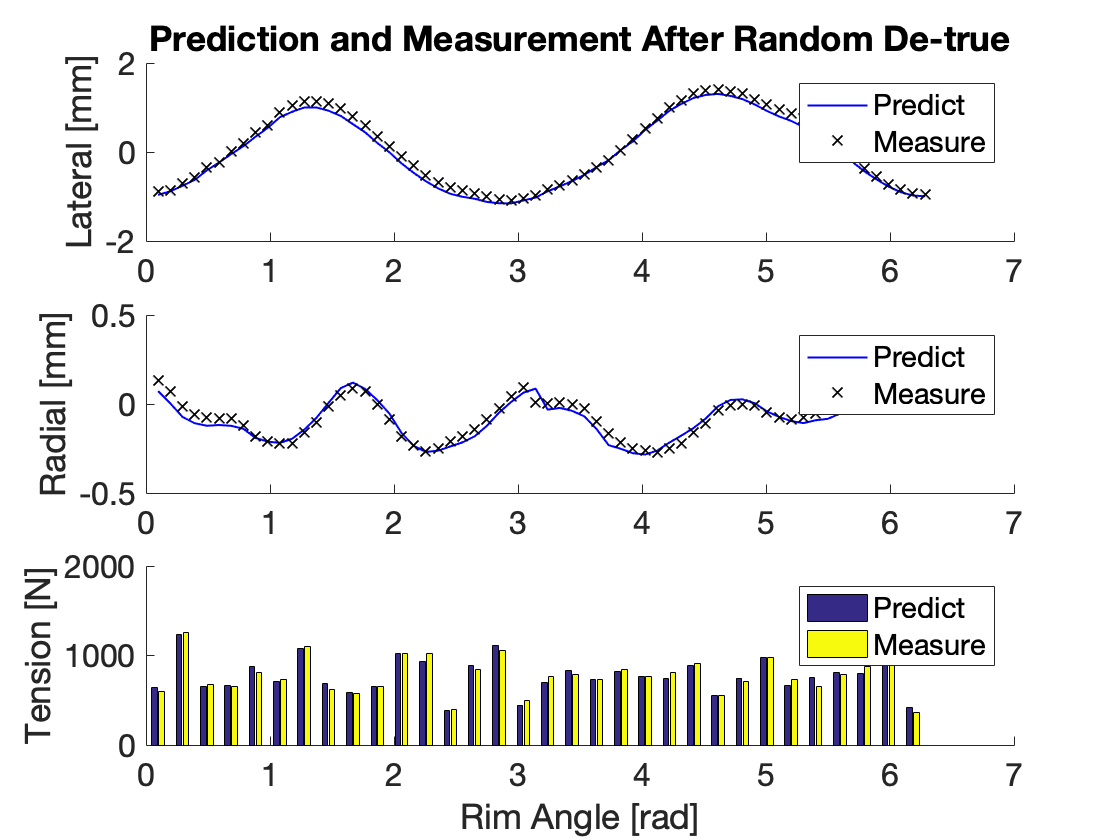
\includegraphics[width=\textwidth]{detune_exp}
        \end{subfigure}
        ~
        \begin{subfigure}[b]{0.45\textwidth}
            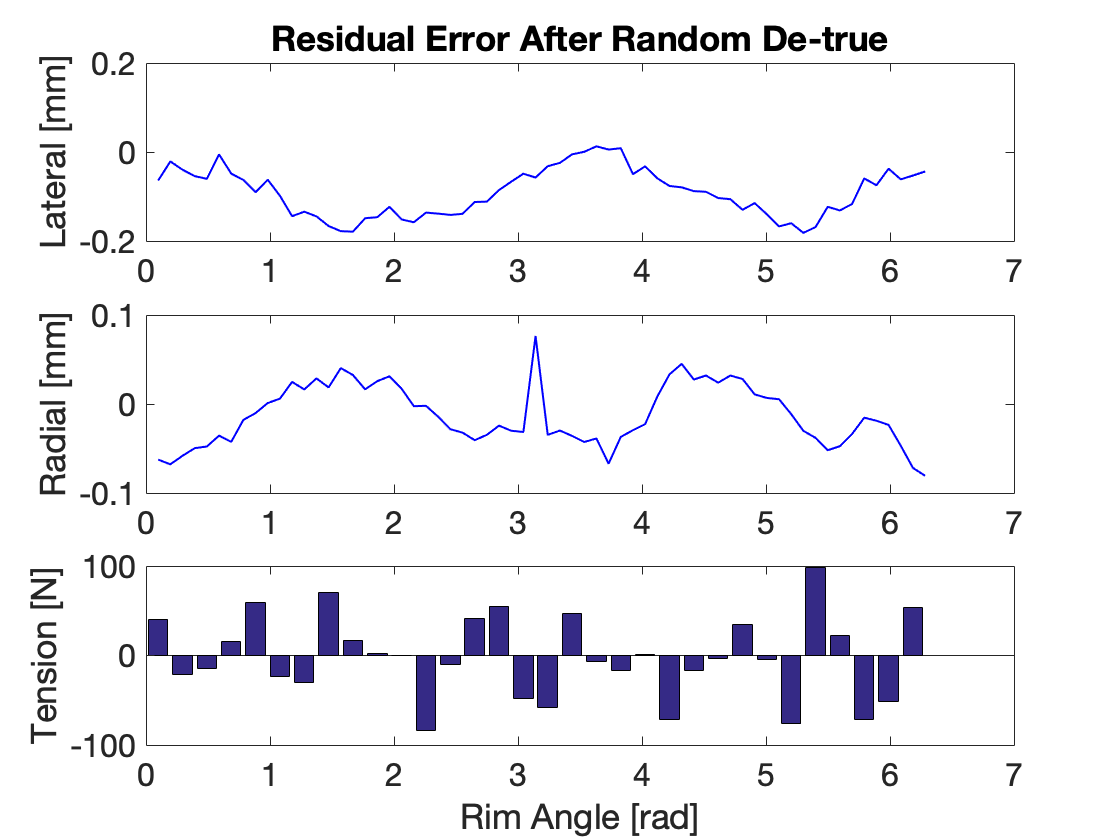
\includegraphics[width=\textwidth]{detune_exp_err}
        \end{subfigure}
\end{figure}
\begin{itemize}
    \item Simulation spoke vector $\bf d$ applied to manually-trued test wheel
    \item Spokes adjusted using lateral feedback
    \item The model predicts the experimental results well; some residual structure is evident
\end{itemize}
\end{frame}

\begin{frame}
\frametitle{Experiment 2: True Test Wheel}
\begin{figure}
        \centering
        \begin{subfigure}[b]{0.45\textwidth}
            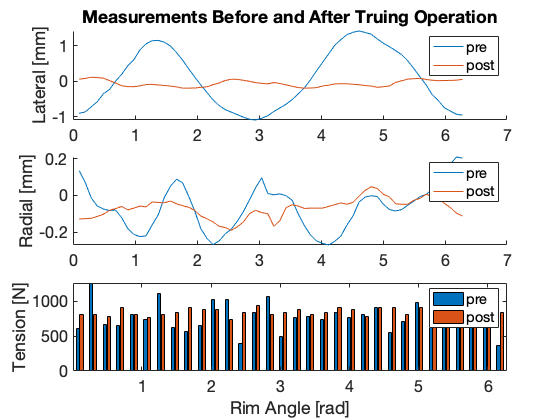
\includegraphics[width=\textwidth]{exp2_pre_post}
        \end{subfigure}
        ~
        \begin{subfigure}[b]{0.45\textwidth}
            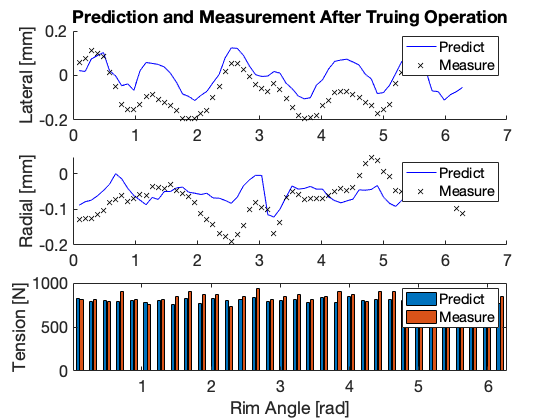
\includegraphics[width=\textwidth]{exp2_predict_measure}
        \end{subfigure}
\end{figure}
Post truing wheel measurements ($\mu \pm \sigma$):
\begin{itemize}
    \item Lateral: $-0.062\pm0.091$mm
    \item Radial: $-0.070\pm0.052$mm
    \item Tension: $849\pm48$N
\end{itemize}
\begin{block}{}

\end{block}
\end{frame}

\begin{frame}
\frametitle{Experiment 3: Iterate Truing Algorithm}
\begin{figure}
        \centering
        \begin{subfigure}[b]{0.45\textwidth}
            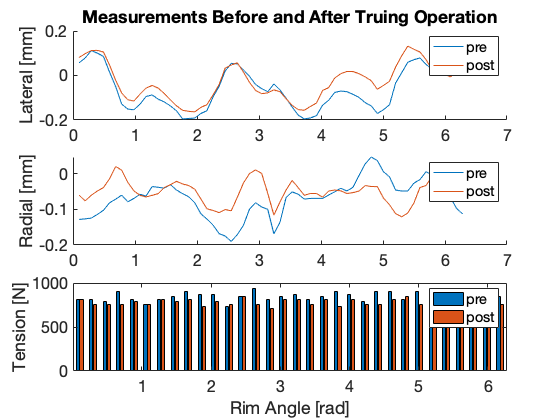
\includegraphics[width=\textwidth]{exp3_pre_post}
        \end{subfigure}
        ~
        \begin{subfigure}[b]{0.45\textwidth}
            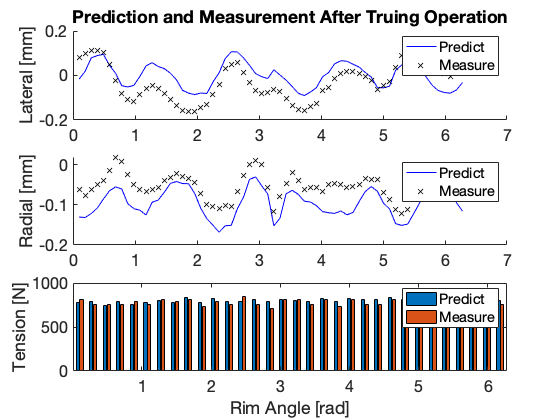
\includegraphics[width=\textwidth]{exp3_predict_measure}
        \end{subfigure}
\end{figure}
Post truing wheel measurements ($\mu \pm \sigma$):
\begin{itemize}
    \item Lateral: $-0.029\pm0.083$mm
    \item Radial: $-0.052\pm0.032$mm
    \item Tension: $781\pm33$N
\end{itemize}
\end{frame}

\section{Conclusions}

\begin{frame}{Conclusions}
      
\end{frame}
      
\section{References}

\begin{frame}{References}
      
\end{frame}

\end{document}  